\frame{
\frametitle{Evaluation}
\begin{center}
%\only<1>{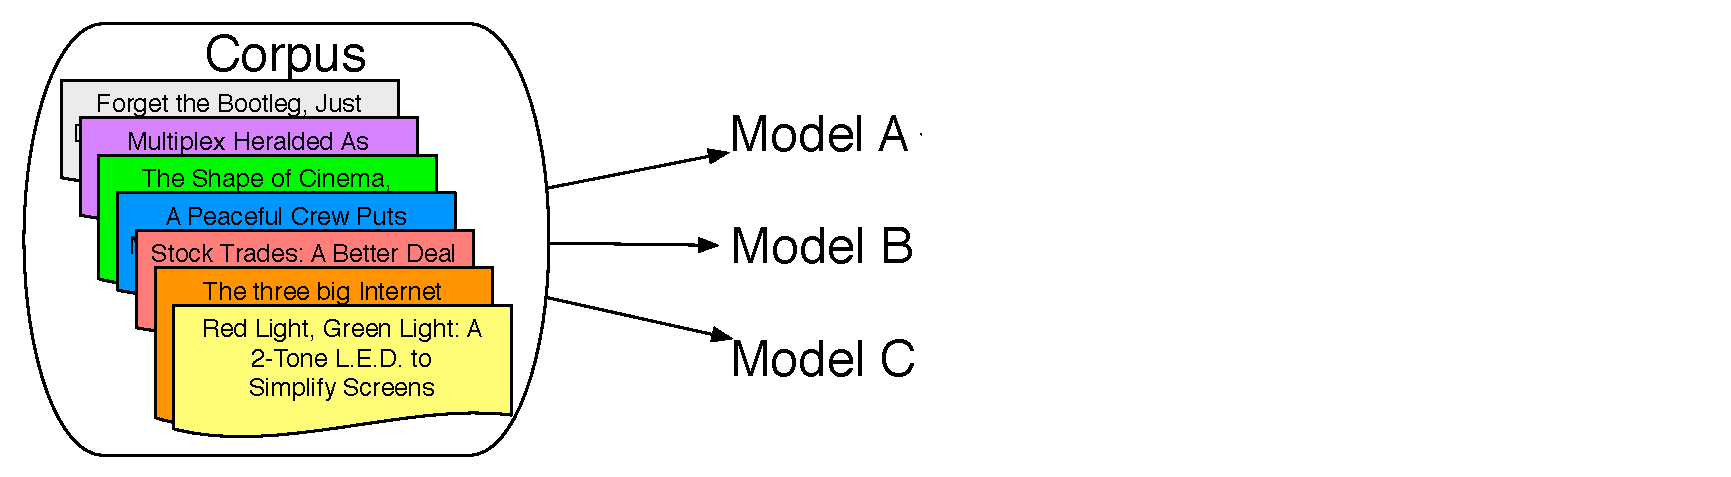
\includegraphics[width=0.9\linewidth]{reading_tea_leaves/figures/heldout_1} }
\only<1>{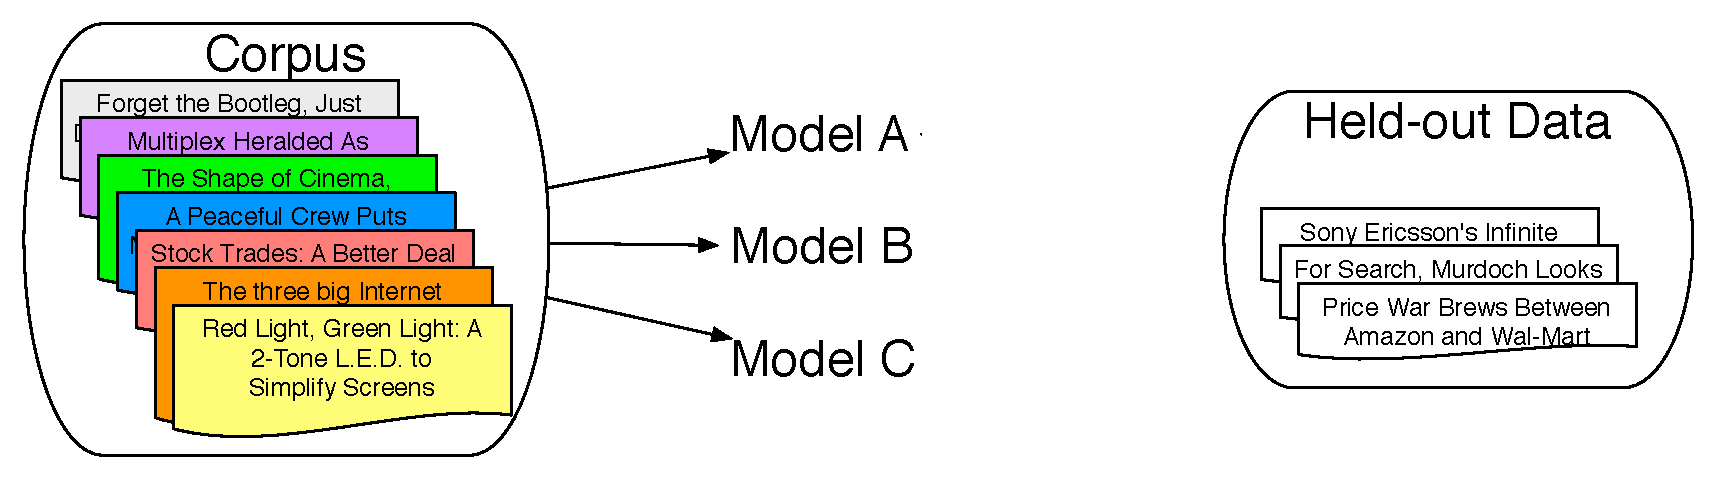
\includegraphics[width=\linewidth]{reading_tea_leaves/figures/heldout_2} }
%\only<3>{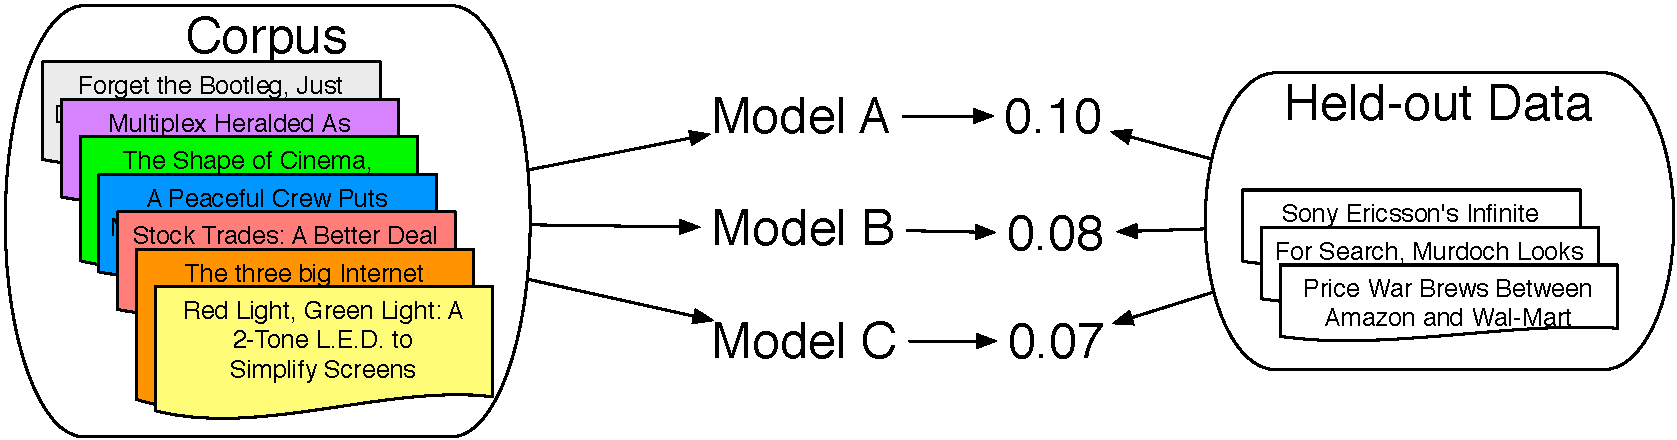
\includegraphics[width=\linewidth]{reading_tea_leaves/figures/heldout_3} }
\only<2>{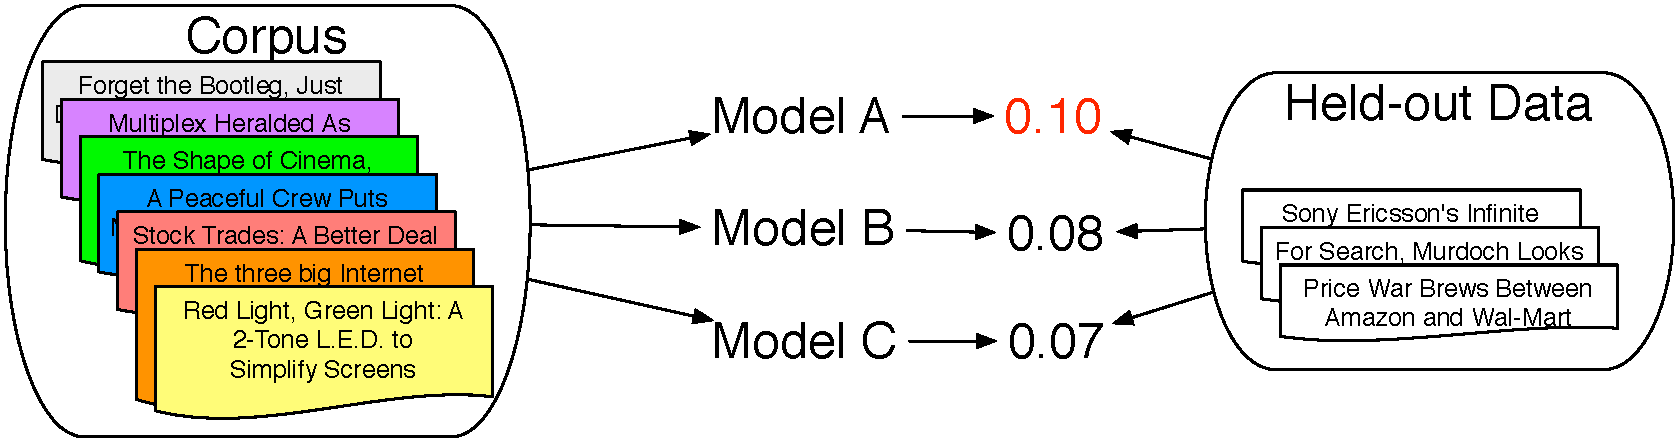
\includegraphics[width=\linewidth]{reading_tea_leaves/figures/heldout_4}  \\
	\large Measures predictive power, not what the topics are}
\end{center}

\begin{center}
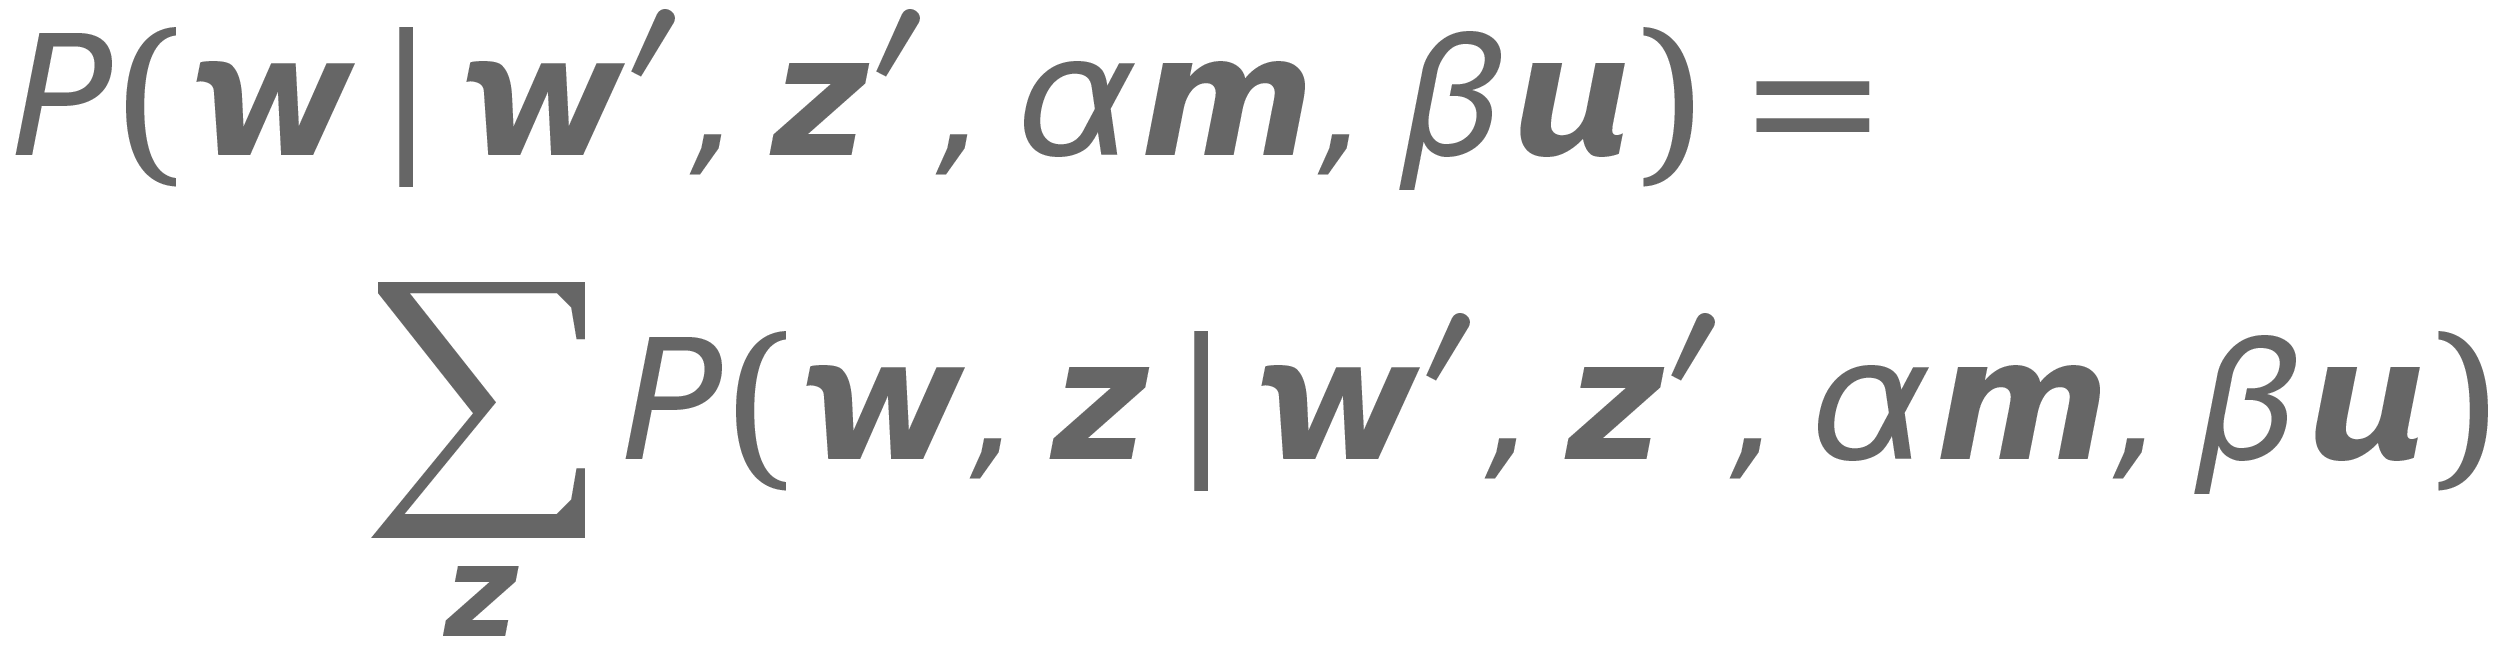
\includegraphics[width=0.5\linewidth]{topic_models/equations/evaluation} \\
How you compute it is important too~\cite{wallach-09b}
\end{center}

}

\frame{
  \frametitle{Word Intrusion}

  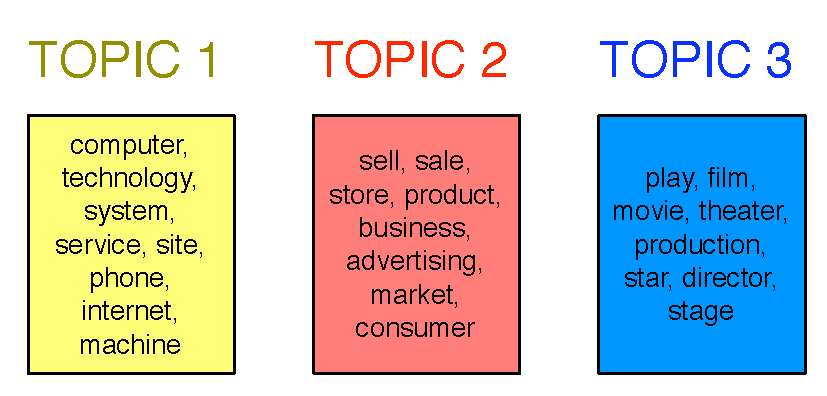
\includegraphics[width=\linewidth]{reading_tea_leaves/figures/nyt_topics_wide}
}


\frame{
  \frametitle{Word Intrusion}

  \begin{enumerate}
    \item Take the highest probability words from a topic

      \begin{block}{Original Topic}
        dog, cat, horse, pig, cow
      \end{block}
\pause
    \item Take a high-probability word from another topic and add it
      \begin{block}{Topic with Intruder}
        dog, cat, \alert<2->{apple}, horse, pig, cow
      \end{block}
\pause
     \item We ask users to find the word that doesn't belong
  \end{enumerate}
\begin{block}{Hypothesis}
If the topics are interpretable, users will consistently choose true intruder
\end{block}
}

\frame{
\frametitle{Word Intrusion}
\begin{center}
\only<1>{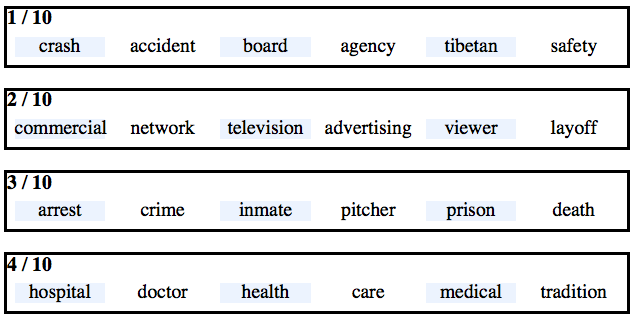
\includegraphics[width=\linewidth]{reading_tea_leaves/tasks/word1}  }
\only<2>{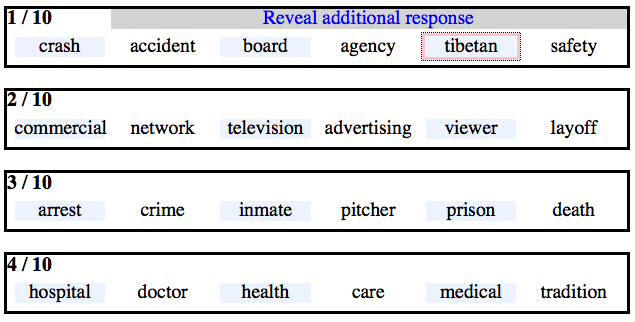
\includegraphics[width=\linewidth]{reading_tea_leaves/tasks/word2}  }
\pause
  \begin{itemize}
    \item Order of words was shuffled
    \item Which intruder was selected varied
    \item Model precision: percentage of users who clicked on intruder
  \end{itemize}

\end{center}
}

\frame{
\frametitle{Word Intrusion: Which Topics are Interpretable?}
  \begin{block}{New York Times, 50 LDA Topics}
    \begin{center}
      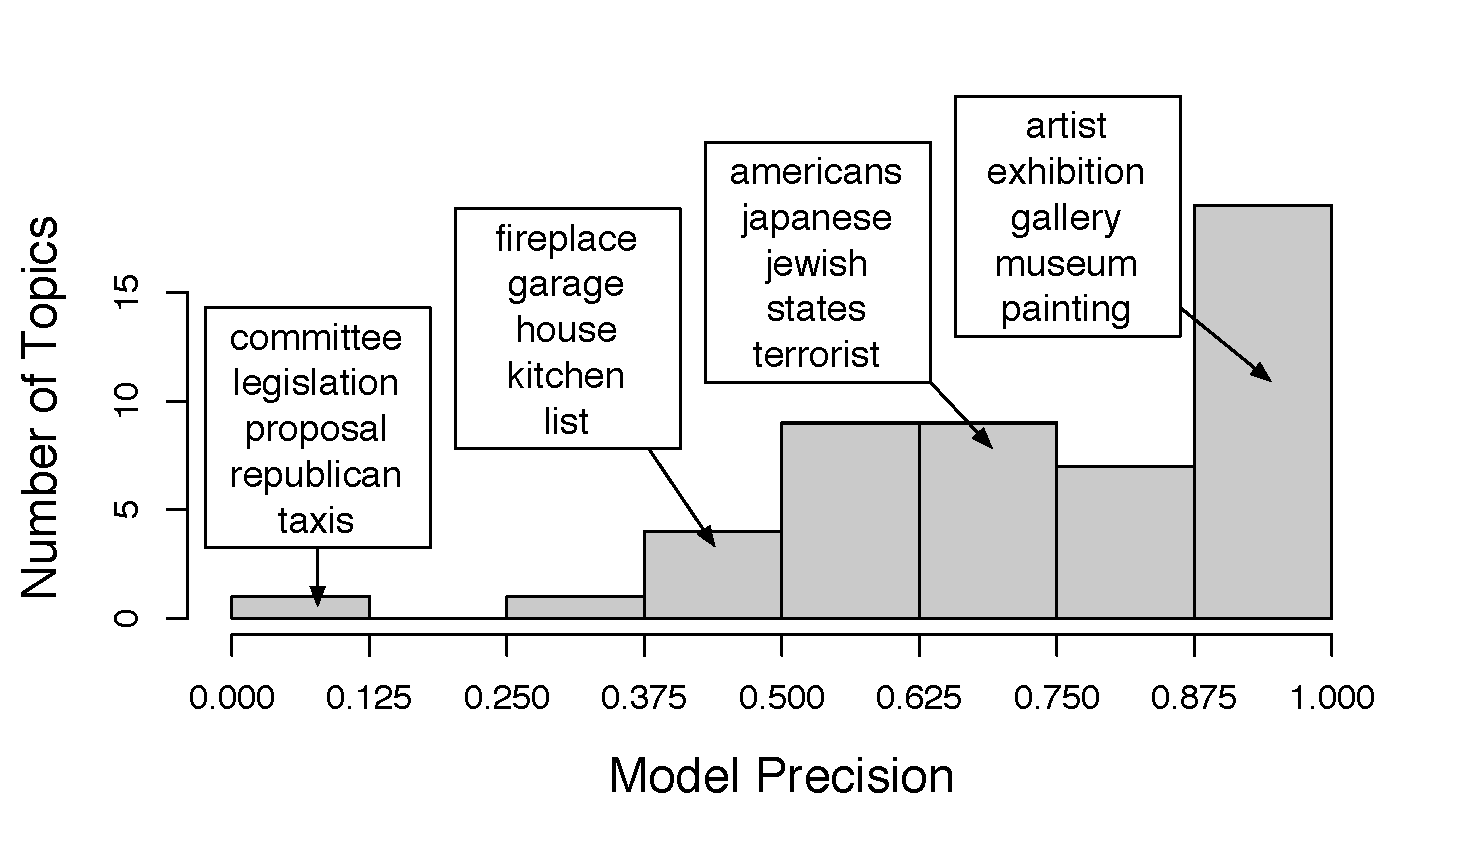
\includegraphics[width=0.8\linewidth]{reading_tea_leaves/figures/topic_precision}
    \end{center}
  \end{block}
  \begin{center}
    Model Precision: percentage of correct intruders found
  \end{center}
}



\frame{

\frametitle{Interpretability and Likelihood}
\begin{center}
\only<1>{Model Precision on New York Times}
\only<2>{Topic Log Odds on Wikipedia}
\end{center}

\begin{columns}
\column{.85\linewidth}
\begin{flushright}
  \only<1>{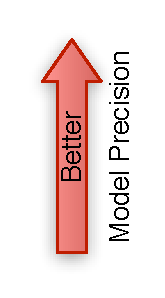
\includegraphics[scale=\graphscale]{reading_tea_leaves/tasks/mp}}
  \only<2>{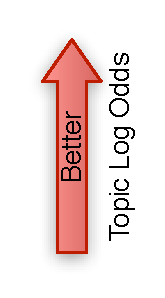
\includegraphics[scale=\graphscale]{reading_tea_leaves/tasks/tlo}}
  \only<1>{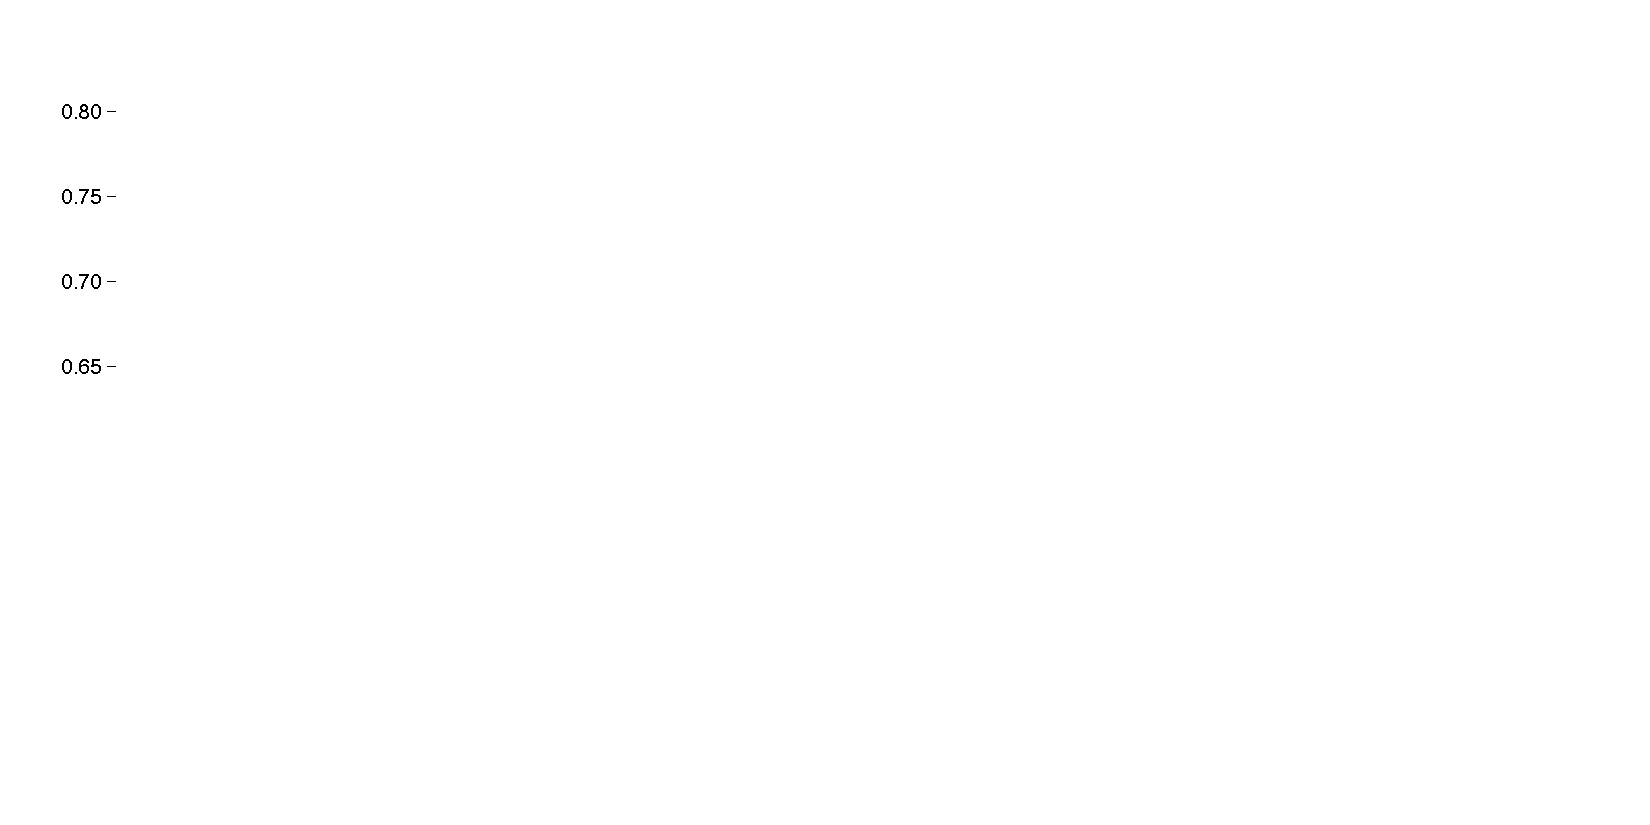
\includegraphics[scale=\graphscale]{reading_tea_leaves/tasks/mp_y}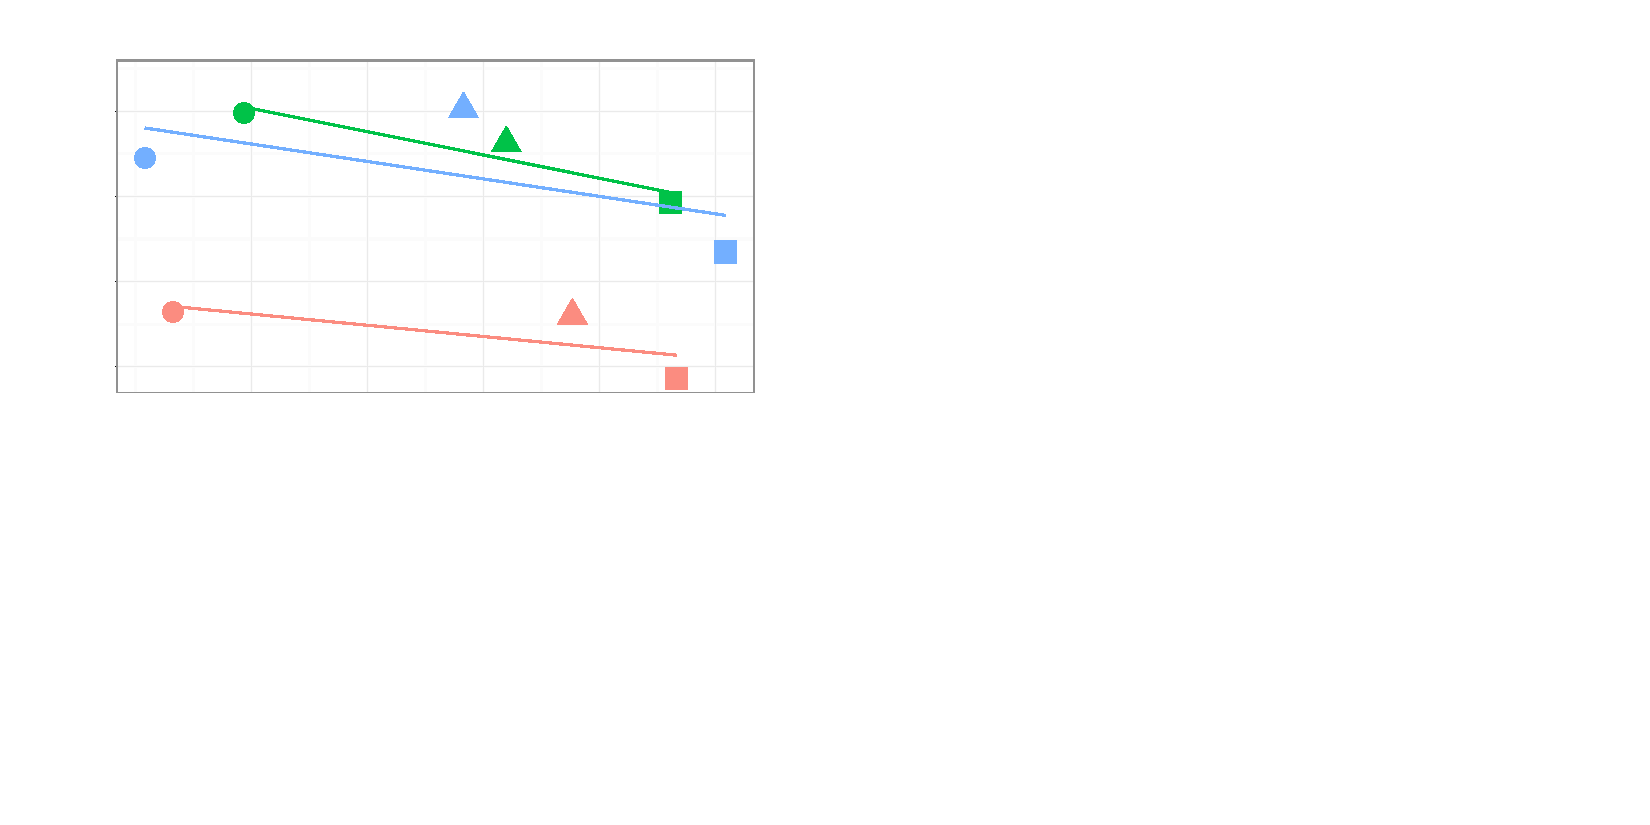
\includegraphics[scale=\graphscale]{reading_tea_leaves/tasks/nyt_mp}}
  \only<2>{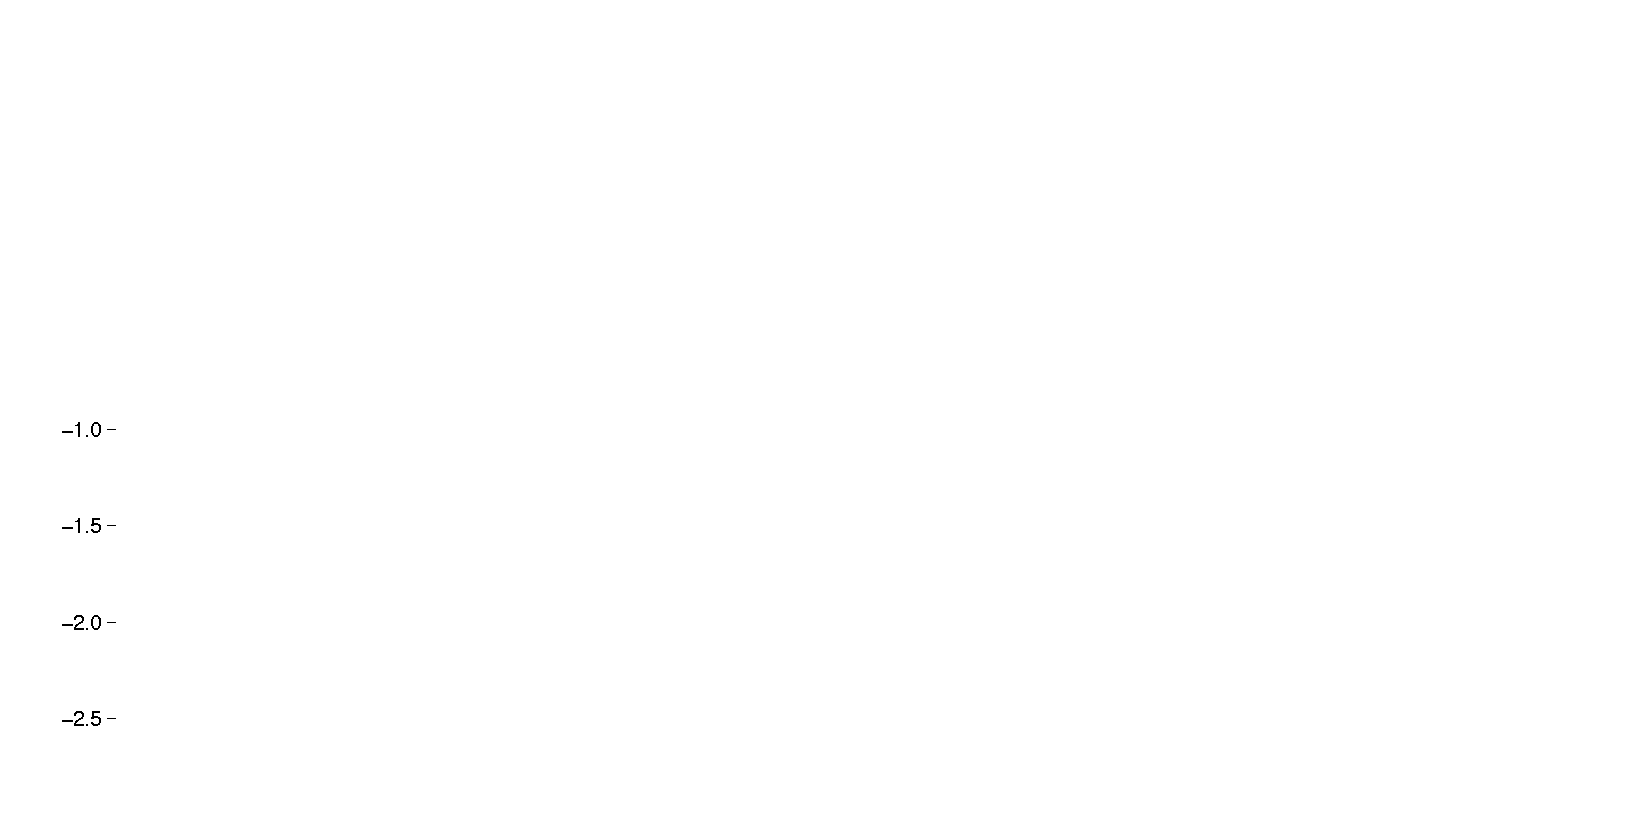
\includegraphics[scale=\graphscale]{reading_tea_leaves/tasks/tlo_y}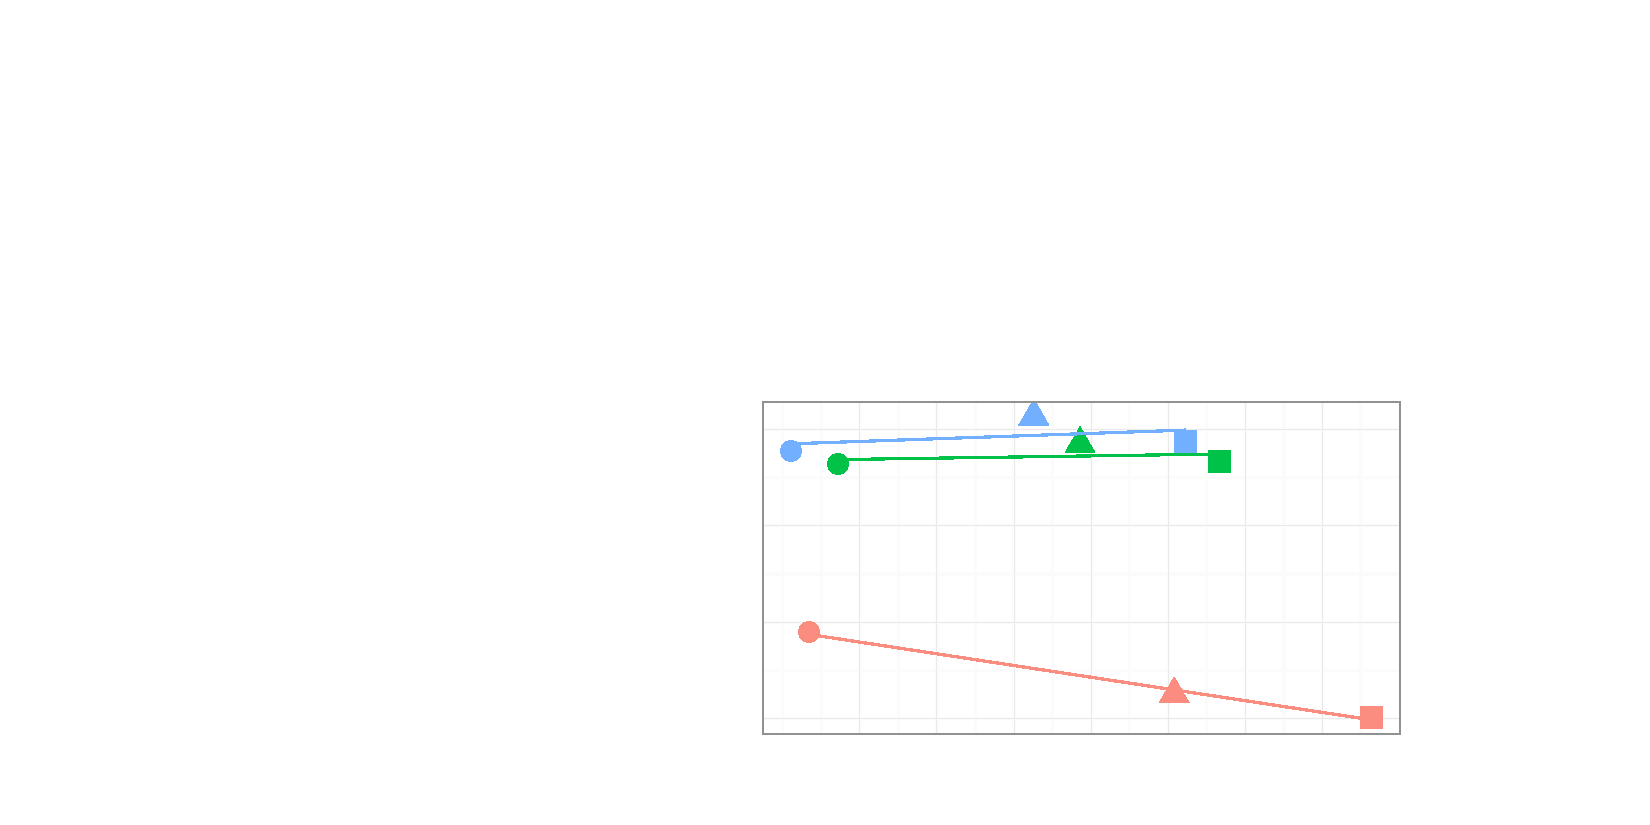
\includegraphics[scale=\graphscale]{reading_tea_leaves/tasks/wiki_tlo}} \\
  \only<1>{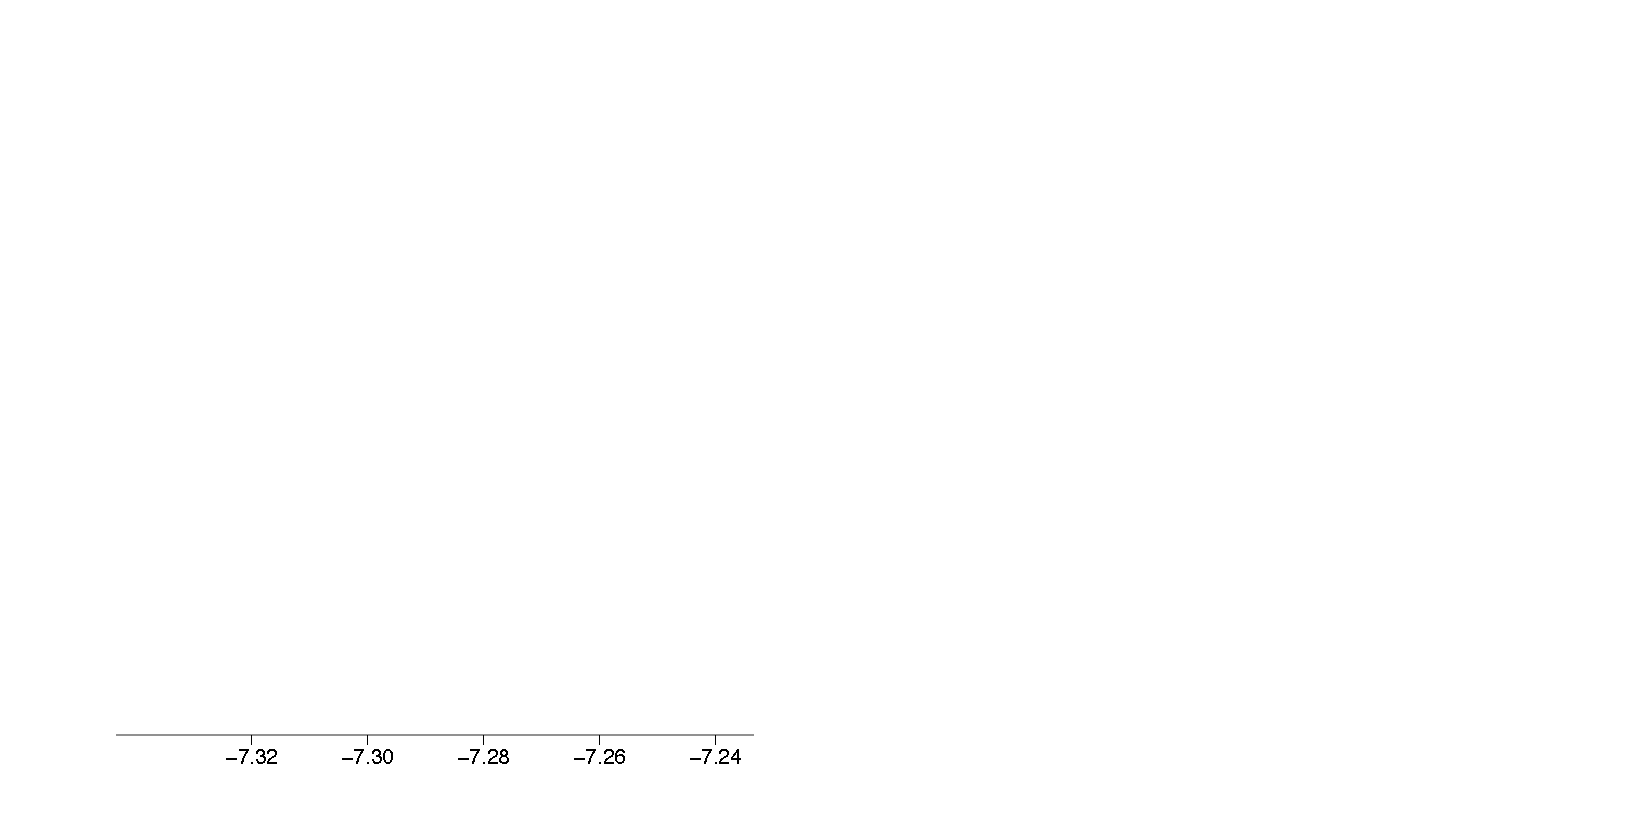
\includegraphics[scale=\graphscale]{reading_tea_leaves/tasks/nyt_x}}
  \only<2>{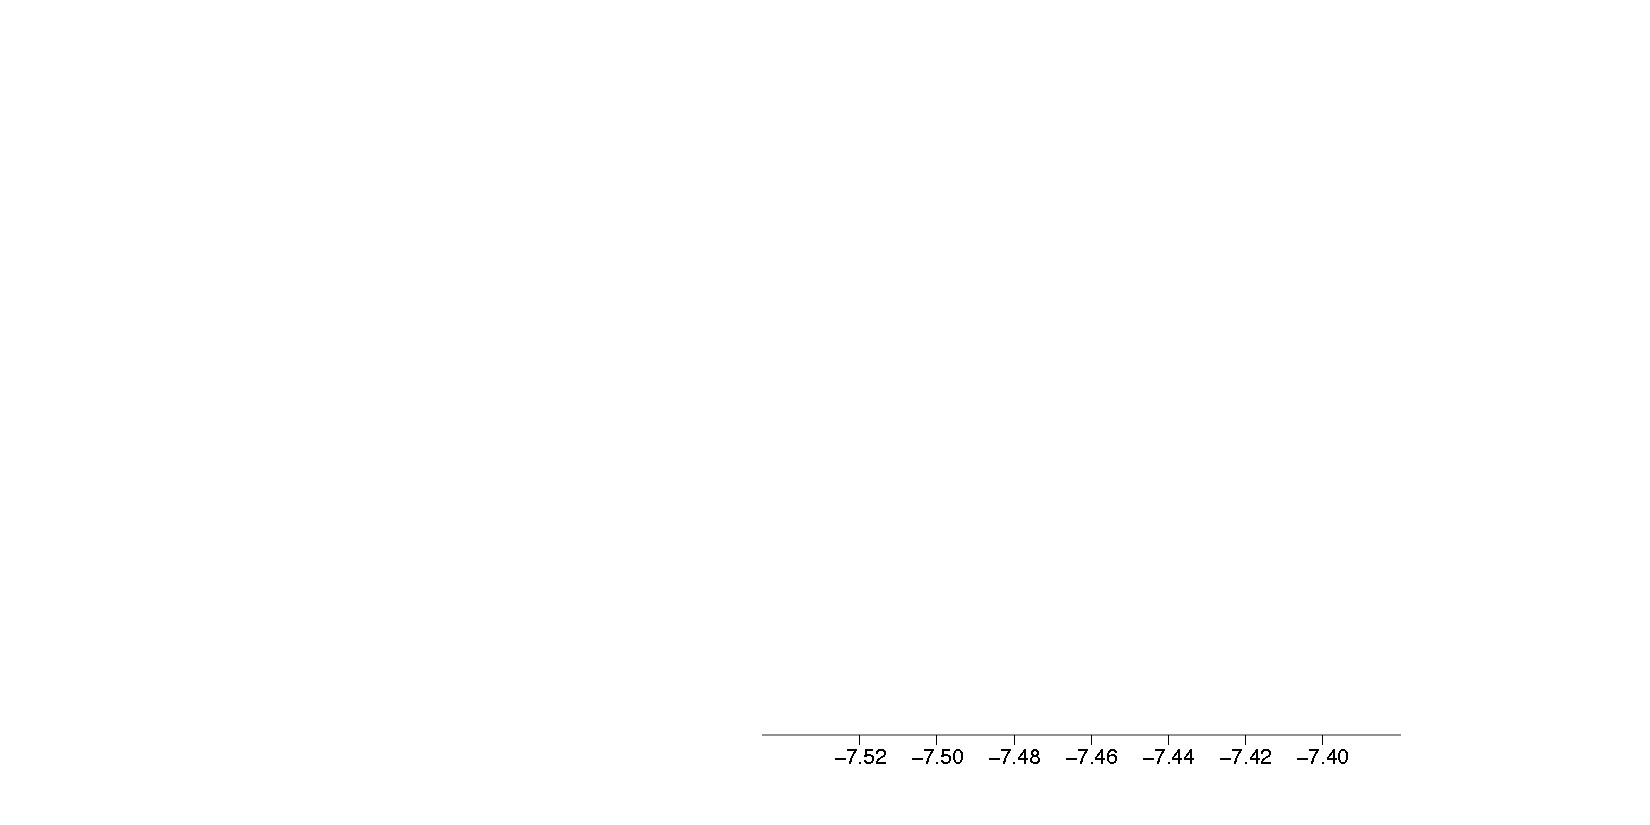
\includegraphics[scale=\graphscale]{reading_tea_leaves/tasks/wiki_x}}
\end{flushright}
\column{.15\linewidth}
  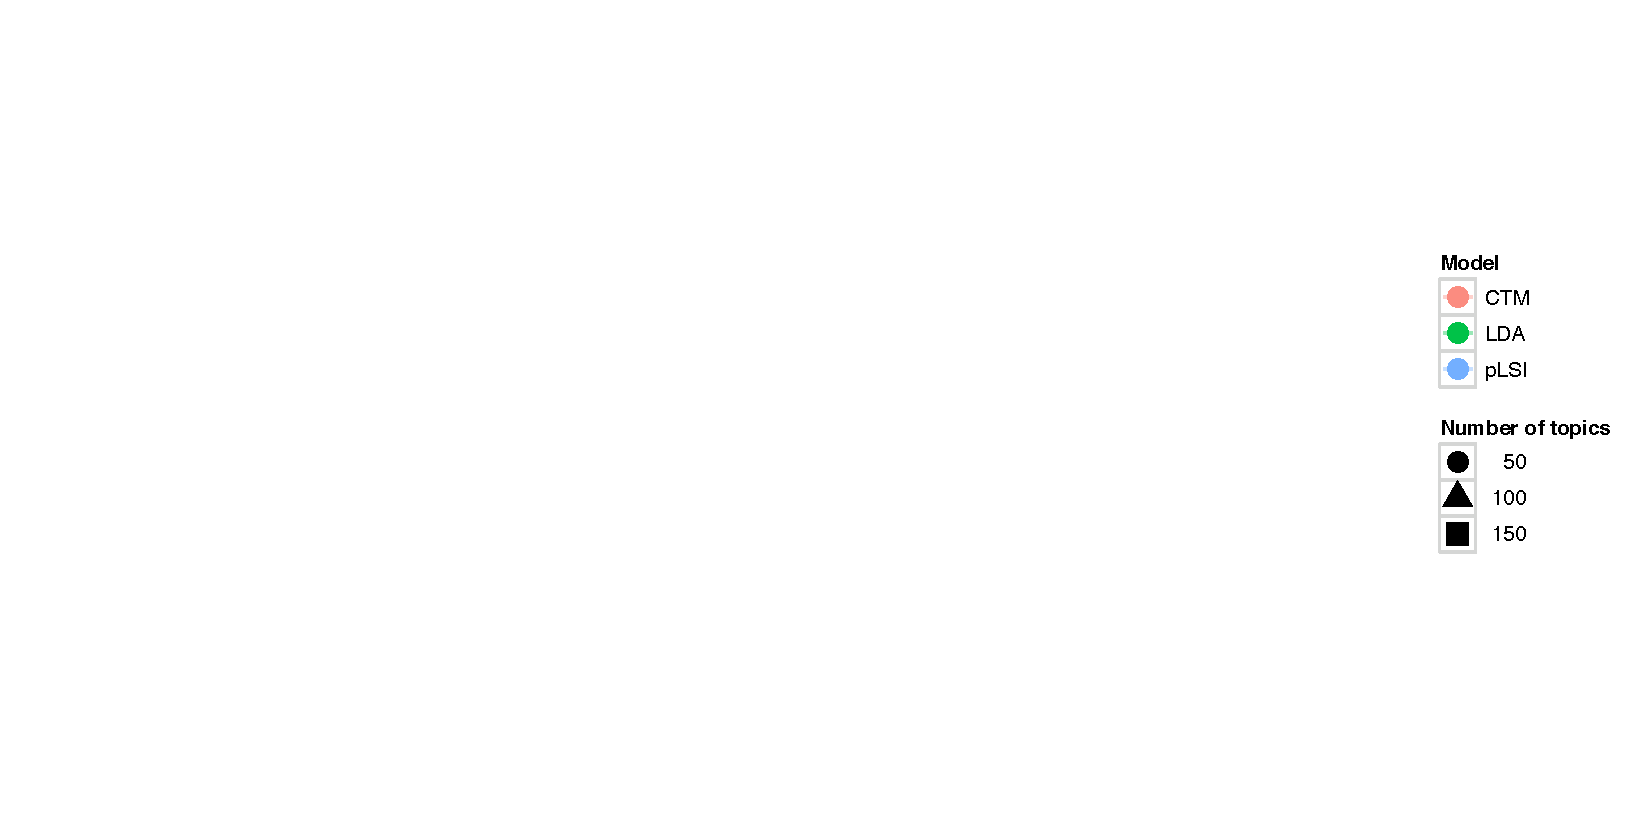
\includegraphics[scale=\graphscale]{reading_tea_leaves/tasks/legend}
\end{columns}
\vspace{-0.75cm}
\begin{center}
  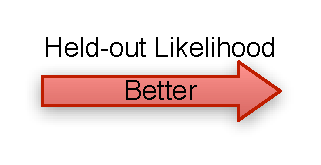
\includegraphics[scale=\graphscale]{reading_tea_leaves/tasks/held-out} \\
\only<1> {within a model, higher likelihood $\not =$ higher interpretability}
\only<2> {across models, higher likelihood $\not =$ higher interpretability}
\end{center}
}


\begin{frame}
  \frametitle{Evaluation Takeaway}

  \begin{itemize}
    \item Measure what you care about~\cite{chang-09c}
      \item If you care about prediction, likelihood is good
\item If you care about a particular task, measure that
    \end{itemize}

\end{frame}
